\documentclass[10.5pt]{ctexart}
\usepackage{xeCJK}%preamble part
\usepackage{graphicx}
\usepackage{indentfirst}
\usepackage[a4paper, inner=1.5cm, outer=1cm, top=2cm, bottom=3cm, bindingoffset=1cm]{geometry}
\usepackage{epstopdf}
\usepackage{multirow}
\usepackage{array}
\usepackage{fontspec}
\usepackage{gensymb}
\usepackage{caption}
\usepackage{subcaption}
\setlength{\extrarowheight}{4pt}
\begin{document}
\title{\textbf{\fontsize{15.75pt}{\baselineskip}{直流电机控制实验报告}}} % 15.75pt is 3 号 in chinese
\author{\fontsize{12pt}{\baselineskip}{数33 赵丰 2013012178 \quad }}
\maketitle
\section{仿真分析}
使用Matlab的Control System Toolbox对所给系统进行分析:所得结果如下:
\textbf{4.1.1} 该直流电机系统模型有两个极点,但极点$-10^{-4}$与主导极点-10相比可忽略,于是直流电机近似为
一阶惯性环节,其阶跃响应曲线为
\begin{figure}[!ht]
\centering
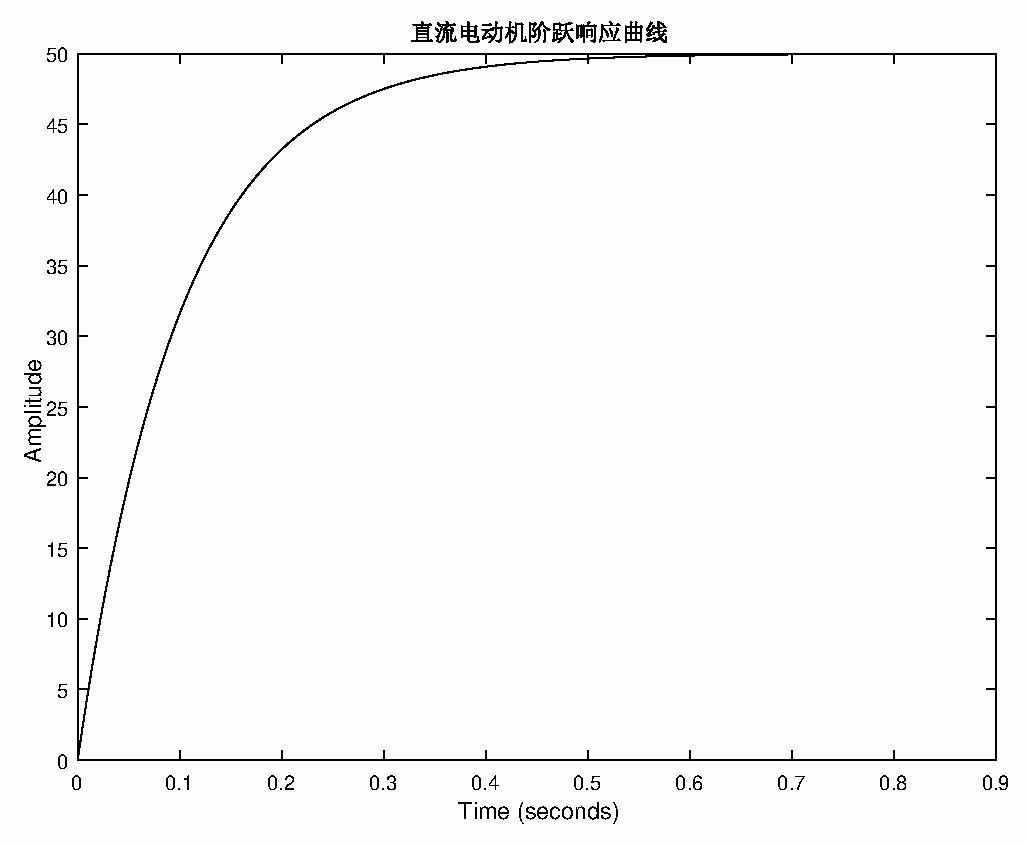
\includegraphics[width=400pt]{step_response_411.eps}
\end{figure}

从图中可以看出,在没有任何控制的情况下(理想情况,无饱和和噪声),直流电机调整时间为秒级。
\newpage
\textbf{4.1.2}
单纯采用比例控制器存在一定局限性,
这一部分的内容来自纸制版的扫描。
\begin{figure}[!ht]
\centering
\includegraphics[width=400pt]{IMG_20161224_201704.jpg}
\end{figure}

采用时域常微分方程的方法可求解该非线性系统,将解的结果与未考虑饱和时的时域响应曲线画在一张图上如下所示:

\begin{figure}[!ht]
\centering
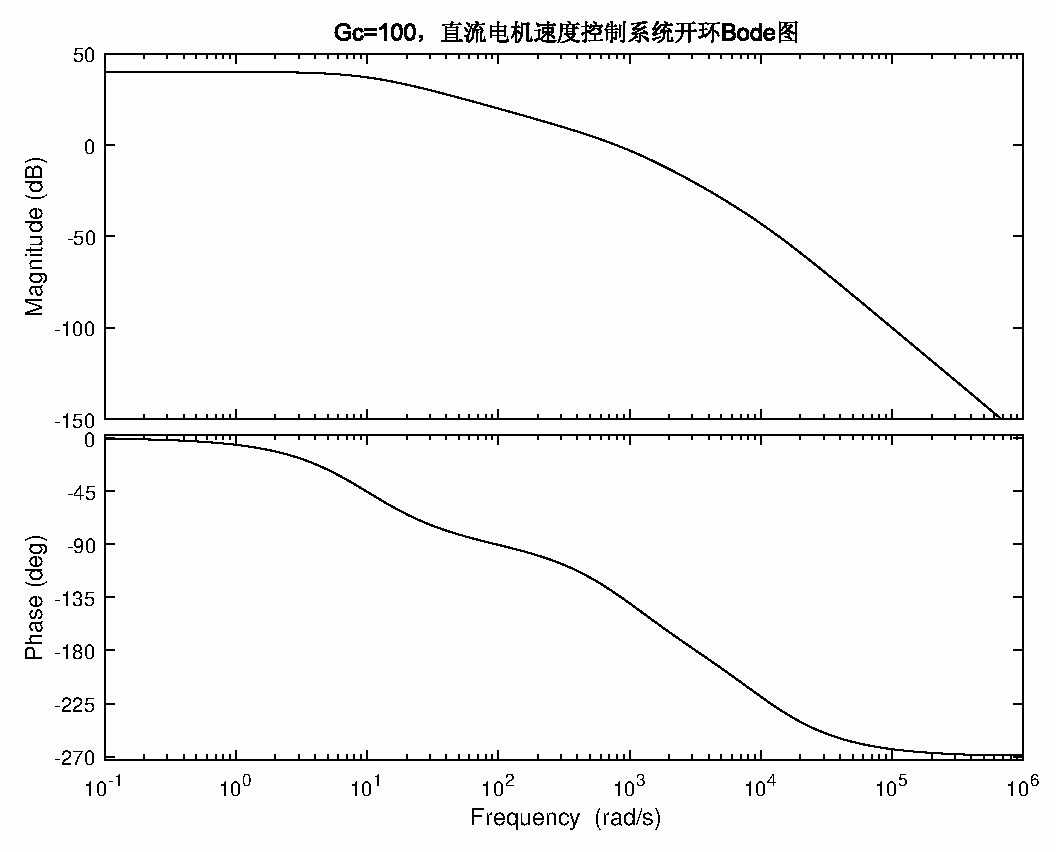
\includegraphics[width=400pt]{bode_plot_4121.eps}
\end{figure}

\begin{figure}[!ht]
\centering
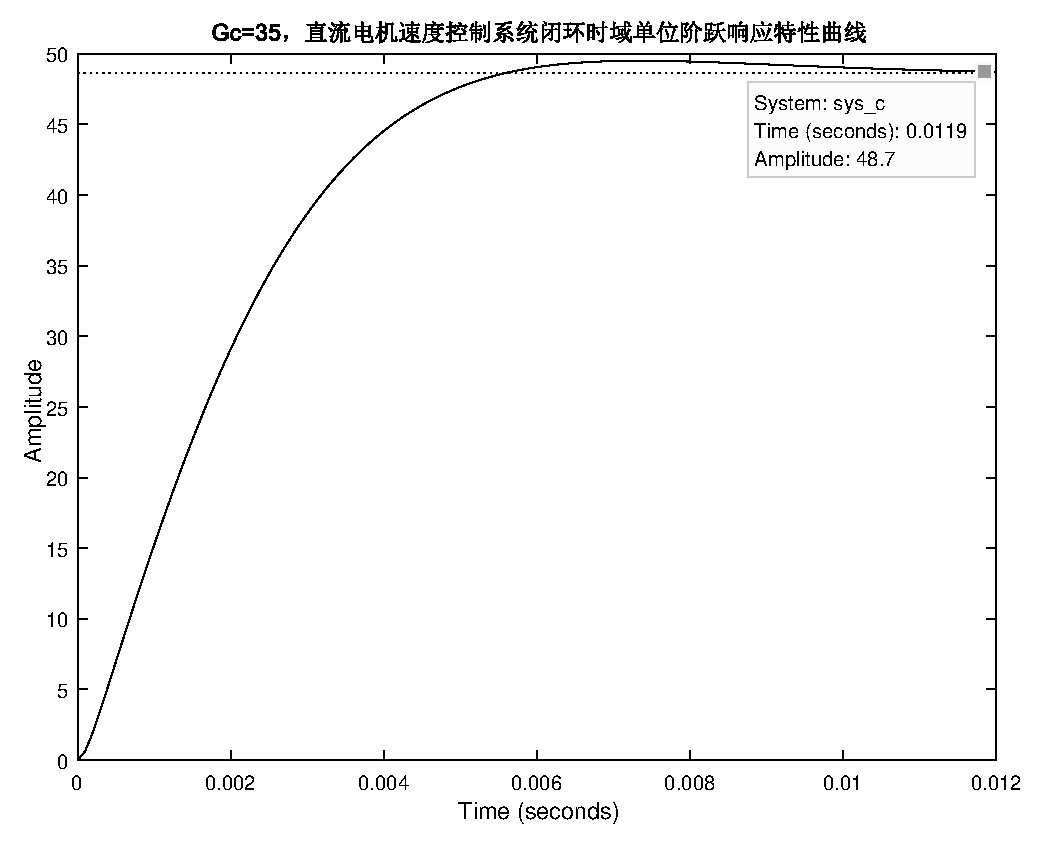
\includegraphics[width=400pt]{step_response_4123.eps}
\end{figure}
\newpage
\begin{figure}[!ht]
\centering
\includegraphics[width=400pt]{step_response_4134.eps}
\end{figure}
\newpage
\textbf{4.1.3}
(1)根据使开环剪切频率尽量大同时对数Bode幅值图以-20dB/1dec的斜率穿过横轴的原则,取速度环Kp=200。
(2)线性系统满足叠加原理,在有负载的情况下,系统可看作一2输入1输出的线性系统,分别求出每一个输入对应的传递函数,由传递函数得到阶跃响应,将两个阶跃响应相加即得到系统在单位阶跃响应下的输出。如下图所示:
\begin{figure}[!ht]
\centering
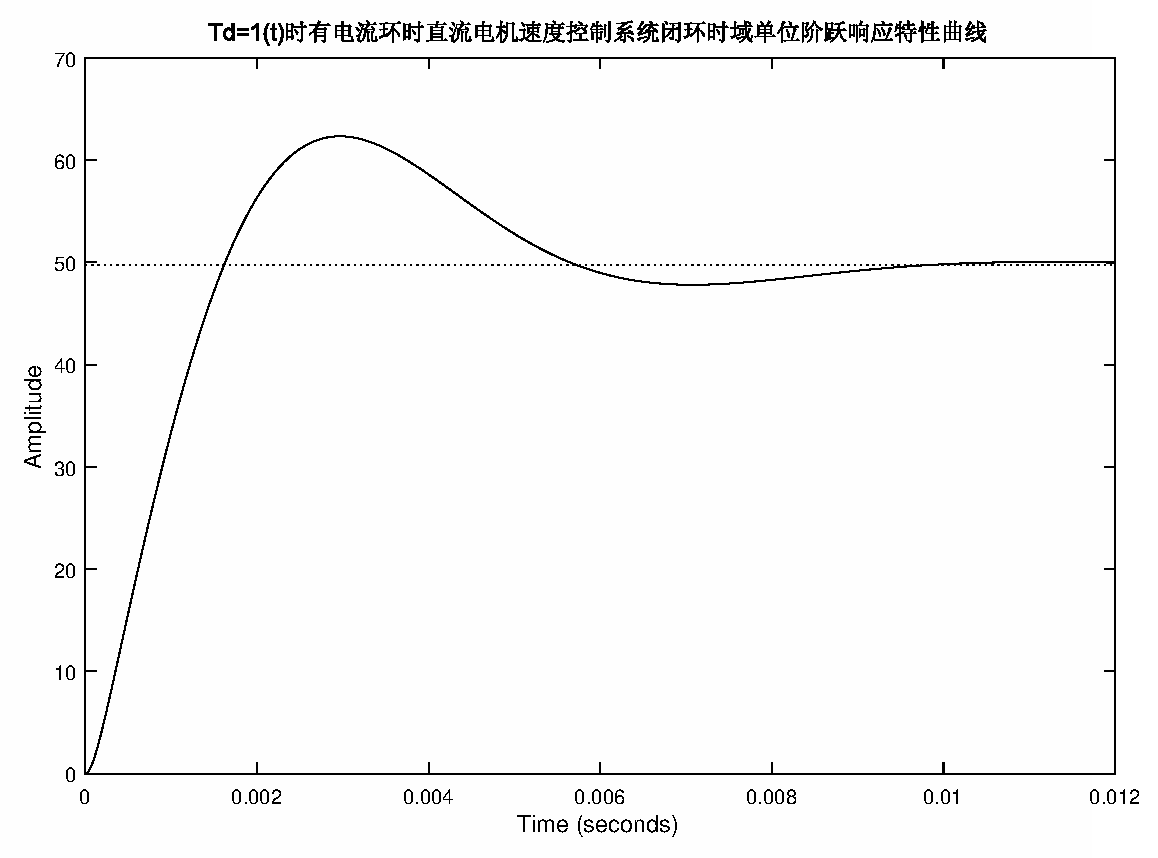
\includegraphics[width=400pt]{step_response_4132.eps}
\end{figure}

无负载时为I型系统,无稳态位置误差,有$T_d$时稳态位置误差来自负载:为0.25/50=0.5\%.
(3)画出位置环$K_p$取值下系统的单位阶跃响应曲线如下所示:
\begin{figure}[!ht]
\centering
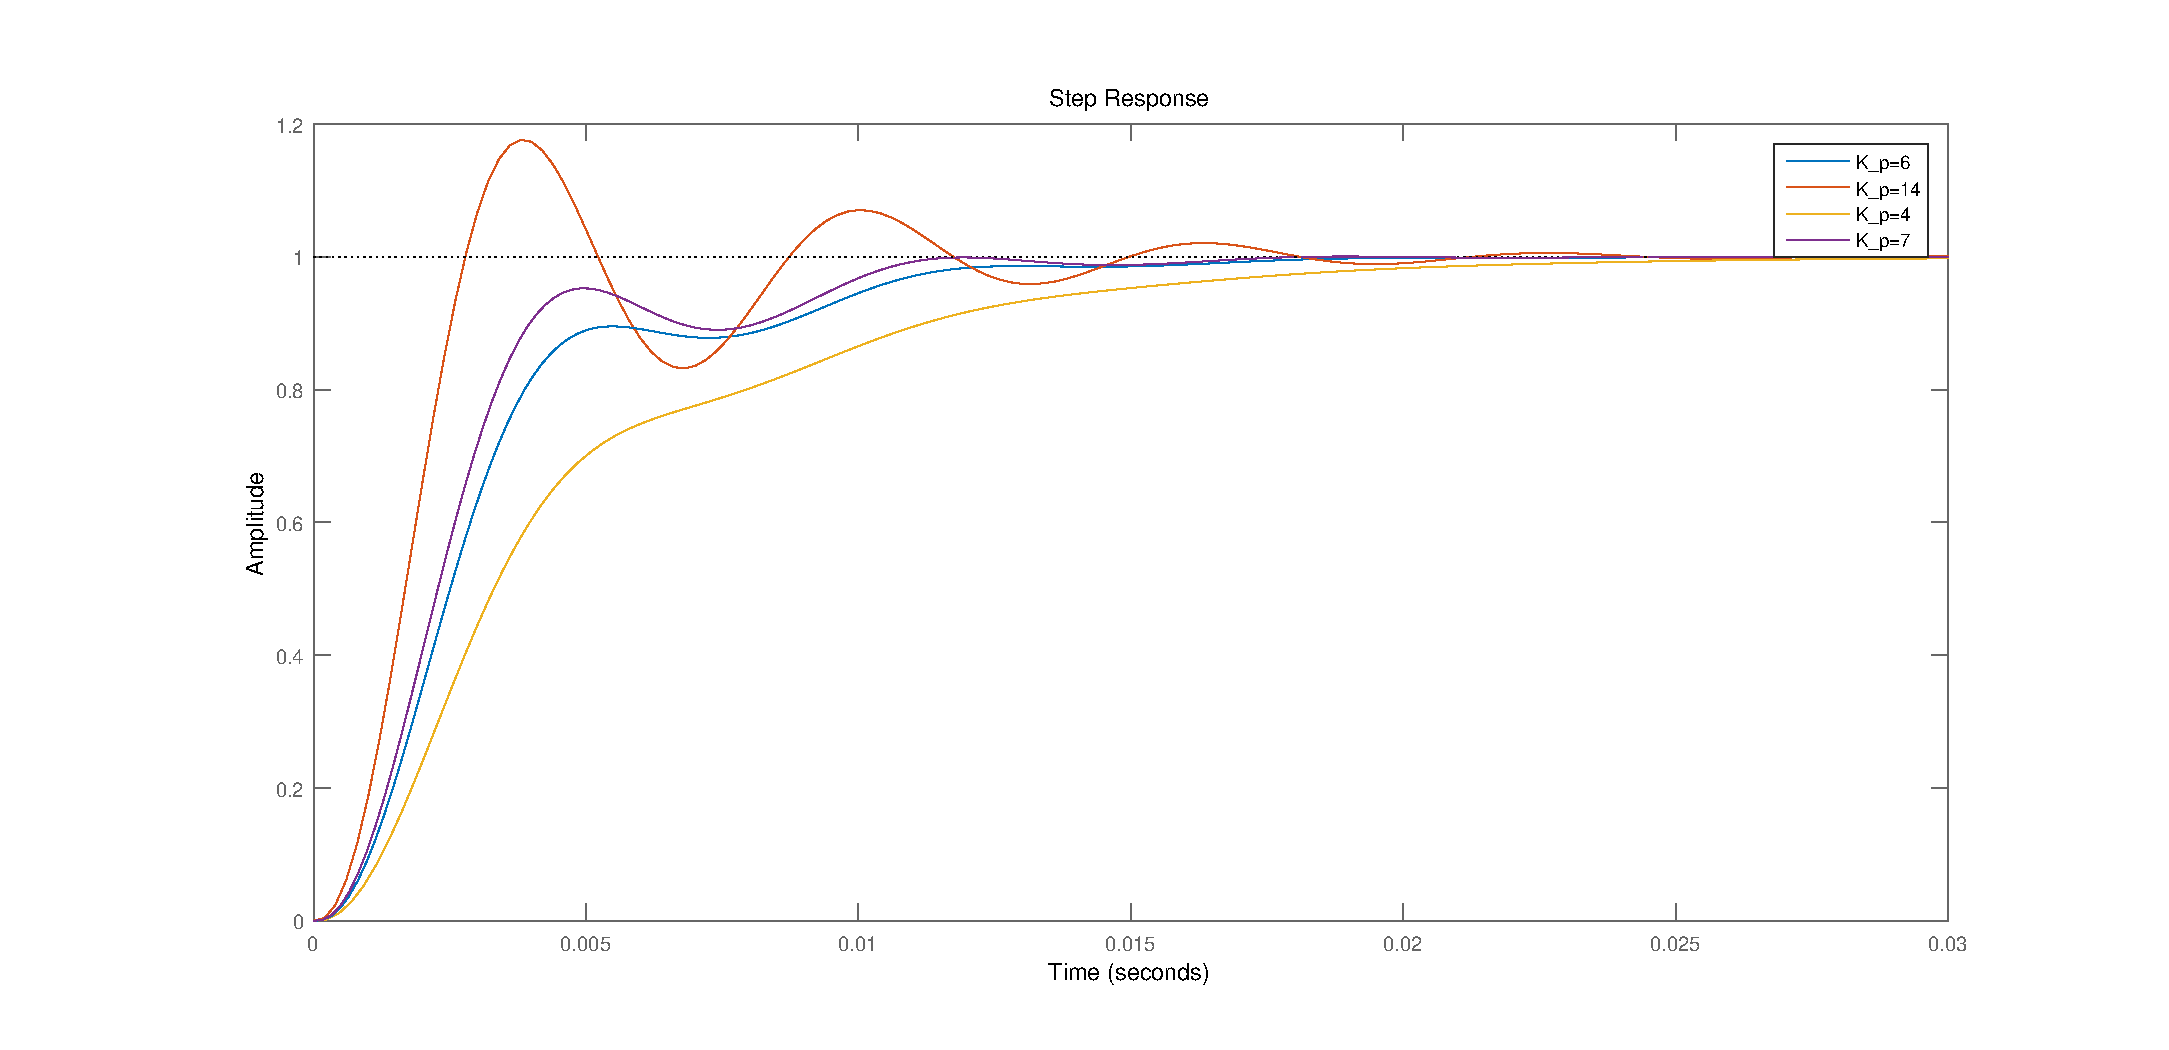
\includegraphics[width=400pt]{Compare.eps}
\end{figure}
通过比较可知应取$K_p=7$
(4)$K_v=350$
\newpage
\section{实验测量}
\textbf{4.2.1:速度环}
根据实验要求调节反馈系数为$F=\frac{1}{3}$,在使用PI控制器的情况下,由于阶跃输入低频成分占主要,PI控制器在低频段幅度增益大,可看作深度负反馈,
$A=\frac{1}{F}=3$,
10-4-A 速度环静态特性测试,分别采用P控制器和PI控制器,输入不同幅值的阶跃信号,以输入控制信号的幅值(有正有负)为横坐标,以输出的电动机转速(由测速发电机转化为电量)作为纵坐标,画出$U_{o}$与$U_{i}$的关系为:
\begin{figure}[!ht]
\centering
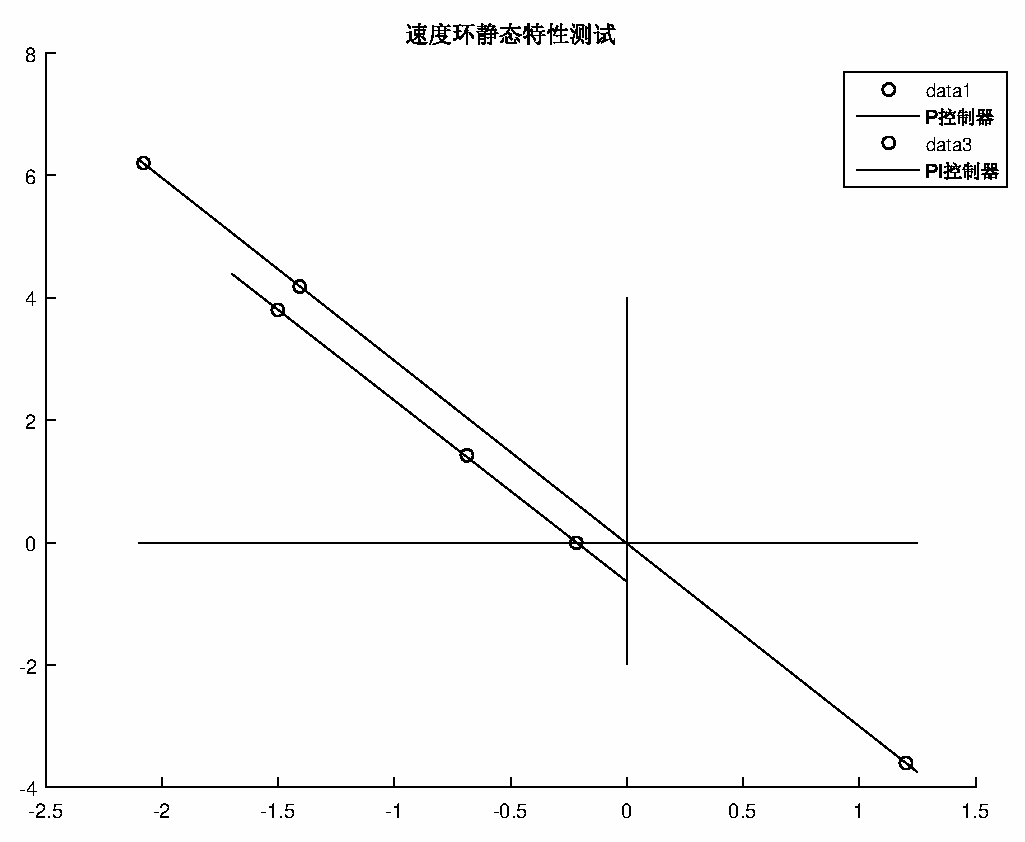
\includegraphics[width=400pt]{vl_static.eps}
\end{figure}
由上图可以看出,对于P控制器,当电压减小到-0.22V时,由于其电压放大倍数较小,运算放大器输出电压经驱动电路后无法使电机克服摩擦阻力的作用,
因此这时输出转速为0.测量其反向死区右端点为$U_{i}=0.29V$左右,因此P控制器存在输入控制量不为零但输出为零的情况。
但对于PI控制器,由于其放大倍数很大,即使输入电压很小也能产生较大的后级驱动电流,因此PI控制器没有死区,表现在图形中即其输入输出特性曲线过原点。由最小二乘法得到拟合直线的斜率P控制器为-2.96,PI控制器为-2.98,均接近理想值-3.\\
10-4-B 速度环动态特性测试,分别对P控制器和PI控制器在接入电路阻值$R_4$一大一小的情况下使用示波器捕捉速度环的时域瞬态响应,如下图所示
\begin{figure}[!ht]
\centering
\caption{P控制,$R_4$较小,无超调,但调整时间较长,约40ms,稳态值为1.8V左右,与输入信号1.5V相比,稳态误差较大}
\includegraphics[width=200pt]{IMG_20161216_100917.jpg}
\end{figure}
\begin{figure}[!ht]
\centering
\caption{P控制,$R_4$较大,虽然调整时间缩短到20ms,但超调太大}
\includegraphics[width=200pt]{IMG_20161216_101251.jpg}
\end{figure}

\begin{figure}[!ht]
\centering
\caption{PI控制,$R_4$较小,超调量大,调整时间较长}
\includegraphics[width=200pt]{IMG_20161216_103304.jpg}
\end{figure}

\begin{figure}[!ht]
\centering
\caption{PI控制,$R_4$较大,超调量小,调整时间较短}
\includegraphics[width=200pt]{IMG_20161216_103650.jpg}
\end{figure}

\newpage
\textbf{4.3:位置环}\\
4.3.1 测定位置环的速度误差系数:系统的位置开环传递函数可近似为$G(s)=\frac{K_v}{s(T_a s+1)}$,若输入一单位阶跃信号,则输出信号为斜坡,其斜率为$K_v$.据此,在系统开环的条件下,用示波器测出输出信号的斜率为$\frac{4.6V}{5s}$,而输入阶跃信号的幅值为0.29V,故$K_v=3.17/s$

4.3.2 位置环闭环动态特性测试,实验发现,在位置环闭环的条件下,速度环采用P控制还是PI控制对实验结果影响不大,因此以下实验测量结果均在速度环采
用PI控制的条件下进行,且位置环的$R_2$调到最大470$\Omega$,以保证位置环的比例因子最大。
若将位置环的0.68$\mu F$的电容短路,即位置环采用P控制,在不同幅值的阶跃信号的激励下,输出波形均近似1阶系统的时域响应曲线,调整时间及稳态电压(由光电编码器测量电机转动角度再经DA转换成模拟电压)如下表所示:
\begin{table}[!ht]
\centering
\caption{位置环采用P控制器动态特性}
\begin{tabular}{ccc}
\hline
输入电压(V) & 调整时间(ms) & 输出电压(V)\\
\hline
-1.0 & 300 & 1.0\\
-2.0 & 600 & 2.0 \\
1.0 & 300 & -1.0\\
2.0 & 600 & -2.0 \\
\hline
\end{tabular}
\end{table}
所测量的输出电压与输入电压反向是由于测量值为反馈回路上的反馈电压。
若将位置环的0.68$\mu F$的电容串联进放大电路中,即位置环采用PI控制,在不同幅值的阶跃信号的激励下,输出波形均近似2阶欠阻尼系统的时域响应曲线,存在超调,且调整时间比起P控制明显偏长,部分结果如下表所示:
\begin{table}[!ht]
\centering
\caption{位置环采用PI控制器动态特性}
\begin{tabular}{ccc}
\hline
输入电压(V) & 调整时间(s) & 输出电压(V)\\
\hline
-1.0 & 1 & 1.0\\
1.0 & 1 & -1.0\\
2.0 & 1.5 & -2.0 \\
\hline
\end{tabular}
\end{table}
若速度环取消反馈,电机会出现自激振荡的现象,测定电机自激振荡的波形近似三角波,两级运放的前级输出方波,无反馈的后级运放作为比较器产生了三角波
因此整个系统此时是一个三角波发生器,测定电机自激振荡的周期为$T=300ms$.
\newpage
4.3.4 测定工作台位移与输入电压的关系:将测试得到的10个点以输入电压为横轴,以工作台位置为纵轴,绘图结果如下:
\begin{figure}[!ht]
\centering
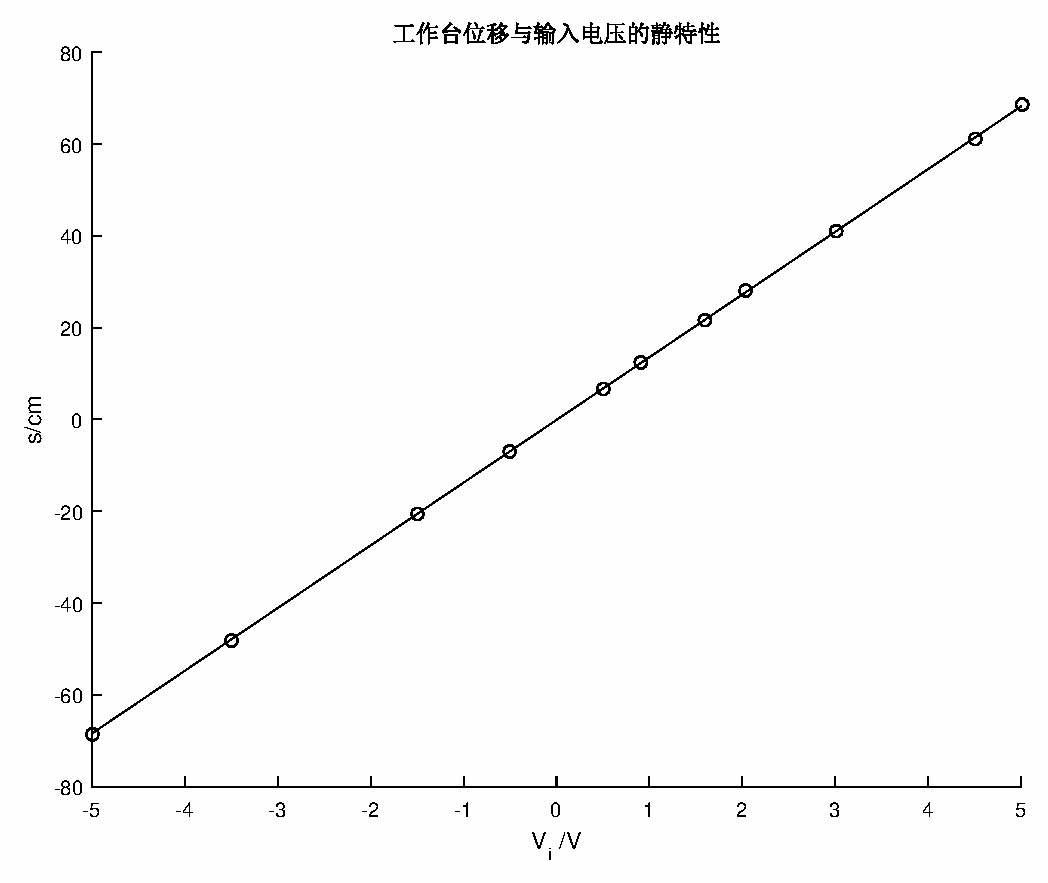
\includegraphics[width=400pt]{static111.eps}
\end{figure}
通过分析直流电机位置伺服系统的方块图可知,速度环是一个二阶系统,而位置环是I型系统,速度误差系数$K_v$的量纲是$s^{-1}$.
若在输入端加上1V的电压信号,其X的位移量根据方块图计算的结果是为12.73cm,根据$s--V_i$图实际测量的结果是13.6cm.

\end{document}